\documentclass[10pt,twocolumn,letterpaper]{article}

\usepackage{cvpr}
\usepackage{times}
\usepackage{epsfig}
\usepackage{graphicx}
\usepackage{amsmath}
\usepackage{amssymb}
\usepackage{subfigure}
\usepackage{epstopdf}
\usepackage{multirow}
\usepackage{graphicx}  %ziqiang
\usepackage{pythonhighlight}   %ziqiang

% Include other packages here, before hyperref.

% If you comment hyperref and then uncomment it, you should delete
% egpaper.aux before re-running latex.  (Or just hit 'q' on the first latex
% run, let it finish, and you should be clear).
\usepackage[breaklinks=true,bookmarks=false]{hyperref}

\cvprfinalcopy % *** Uncomment this line for the final submission

\def\cvprPaperID{****} % *** Enter the CVPR Paper ID here
\def\httilde{\mbox{\tt\raisebox{-.5ex}{\symbol{126}}}}

% Pages are numbered in submission mode, and unnumbered in camera-ready
%\ifcvprfinal\pagestyle{empty}\fi
\setcounter{page}{1}
\begin{document}

%%%%%%%%% TITLE
\title{CMPE 264 - Project Assignment 2}

\author{Yanan Xie\\
{\tt\small yaxie@ucsc.edu}
% For a paper whose authors are all at the same institution,
% omit the following lines up until the closing ``}''.
% Additional authors and addresses can be added with ``\and'',
% just like the second author.
% To save space, use either the email address or home page, not both
\and
Ziqiang Wang\\
{\tt\small zwang232@ucsc.edu}
}

\maketitle
%\thispagestyle{empty}

%%%%%%%%% ABSTRACT

%%%%%%%%% BODY TEXT
\section{Camera radiometric calibration}

\section{Take the pictures}

We use the same camera and lens take 3 pictures as shown in Figure \ref{fig:pictures}. We placed some objects in the front and also left enough distant background.
\begin{figure}[t]
\centering
\subfigure[Image 1]{
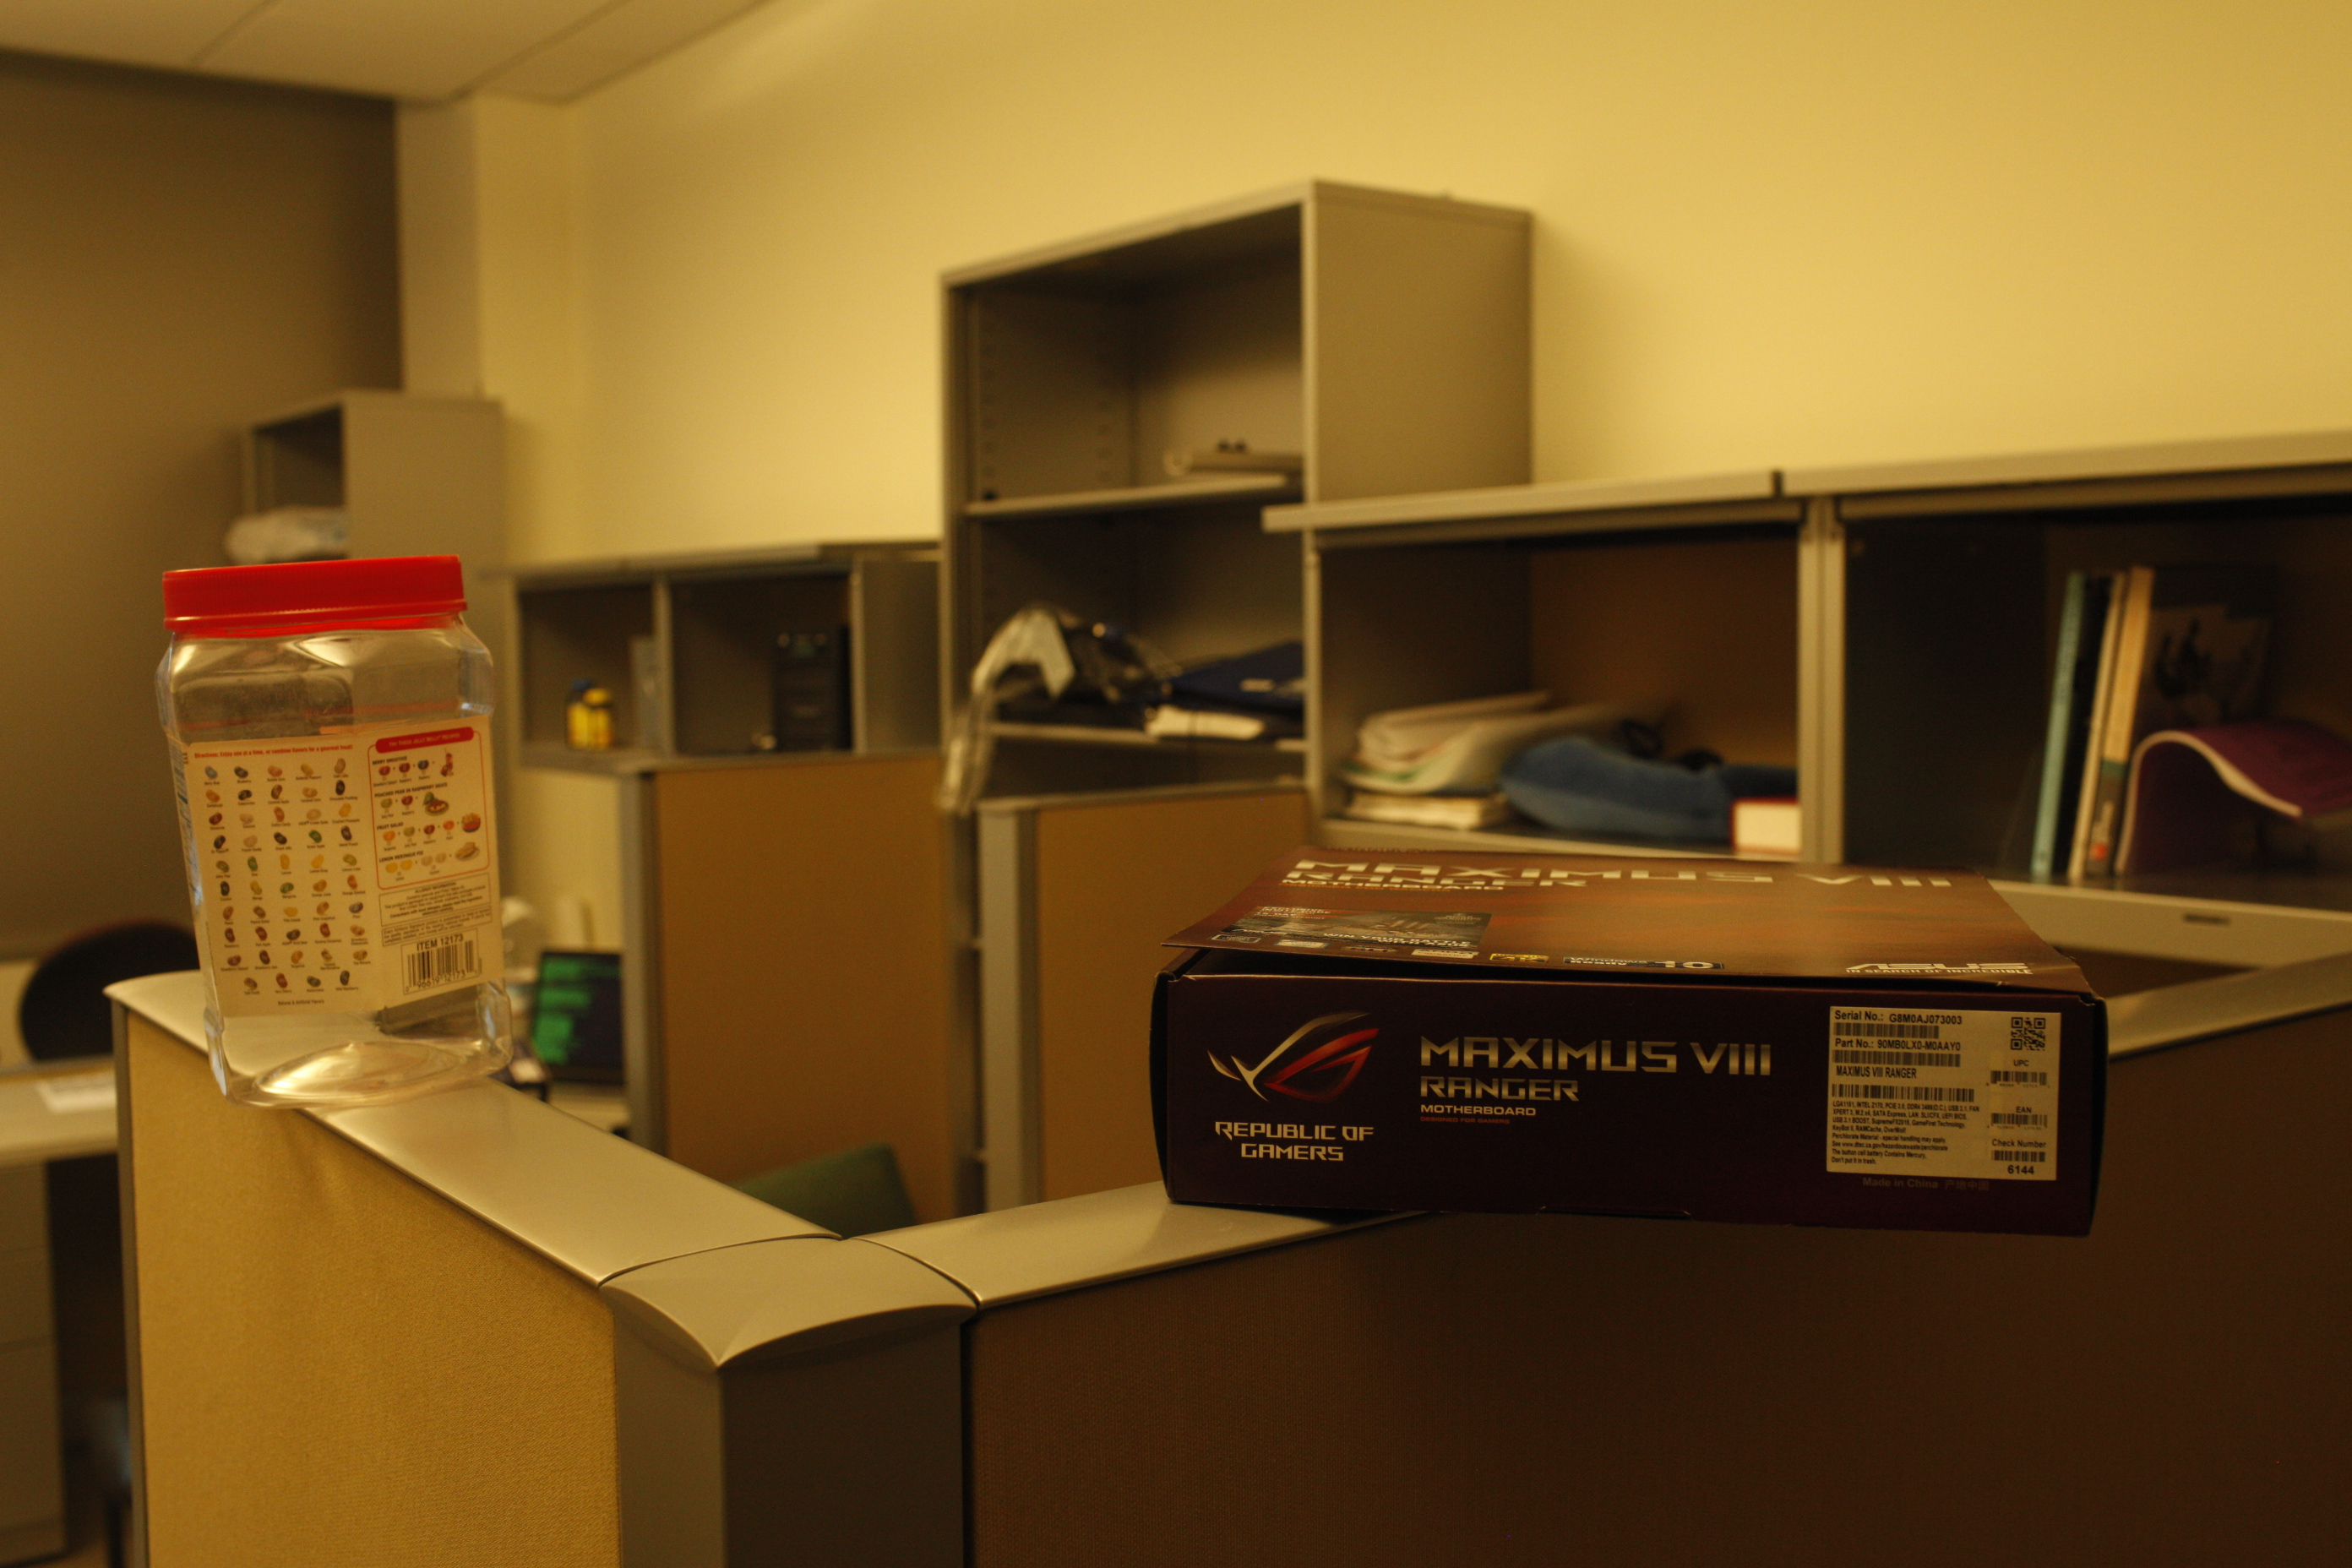
\includegraphics[width=.3\columnwidth]{images/multiview/p1}
}
\subfigure[Image 2]{
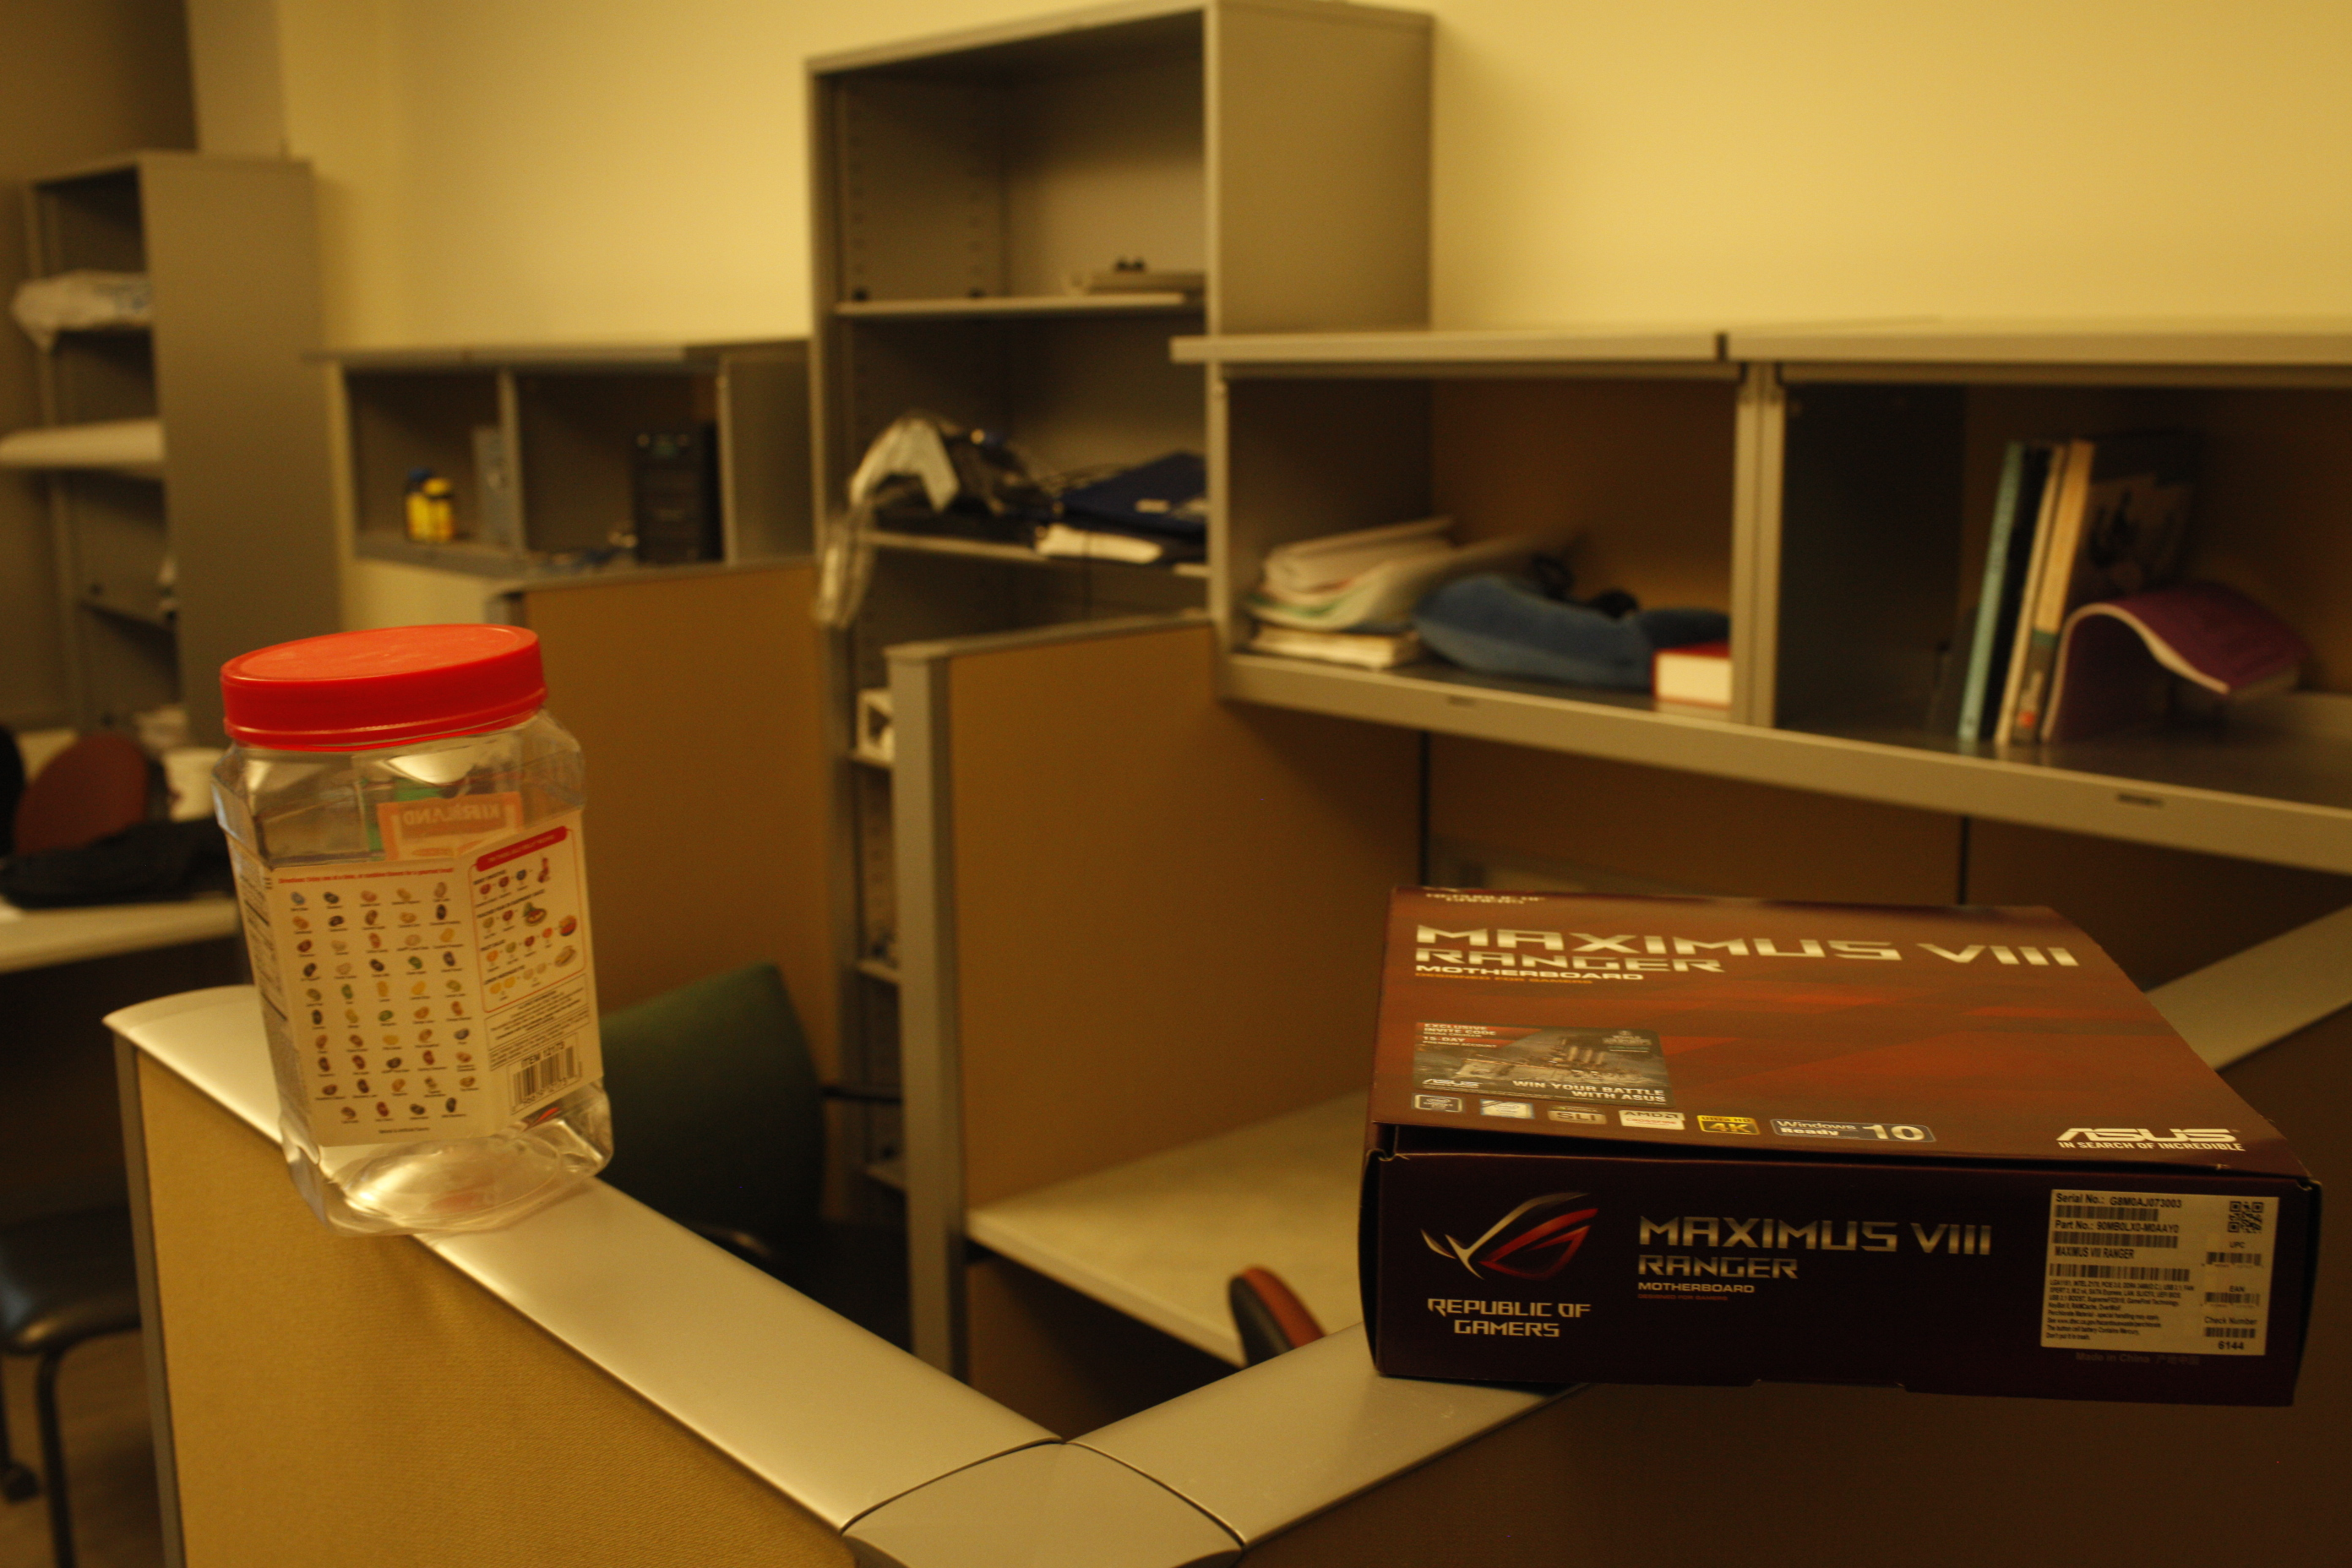
\includegraphics[width=.3\columnwidth]{images/multiview/p2}
}
\subfigure[Image 3]{
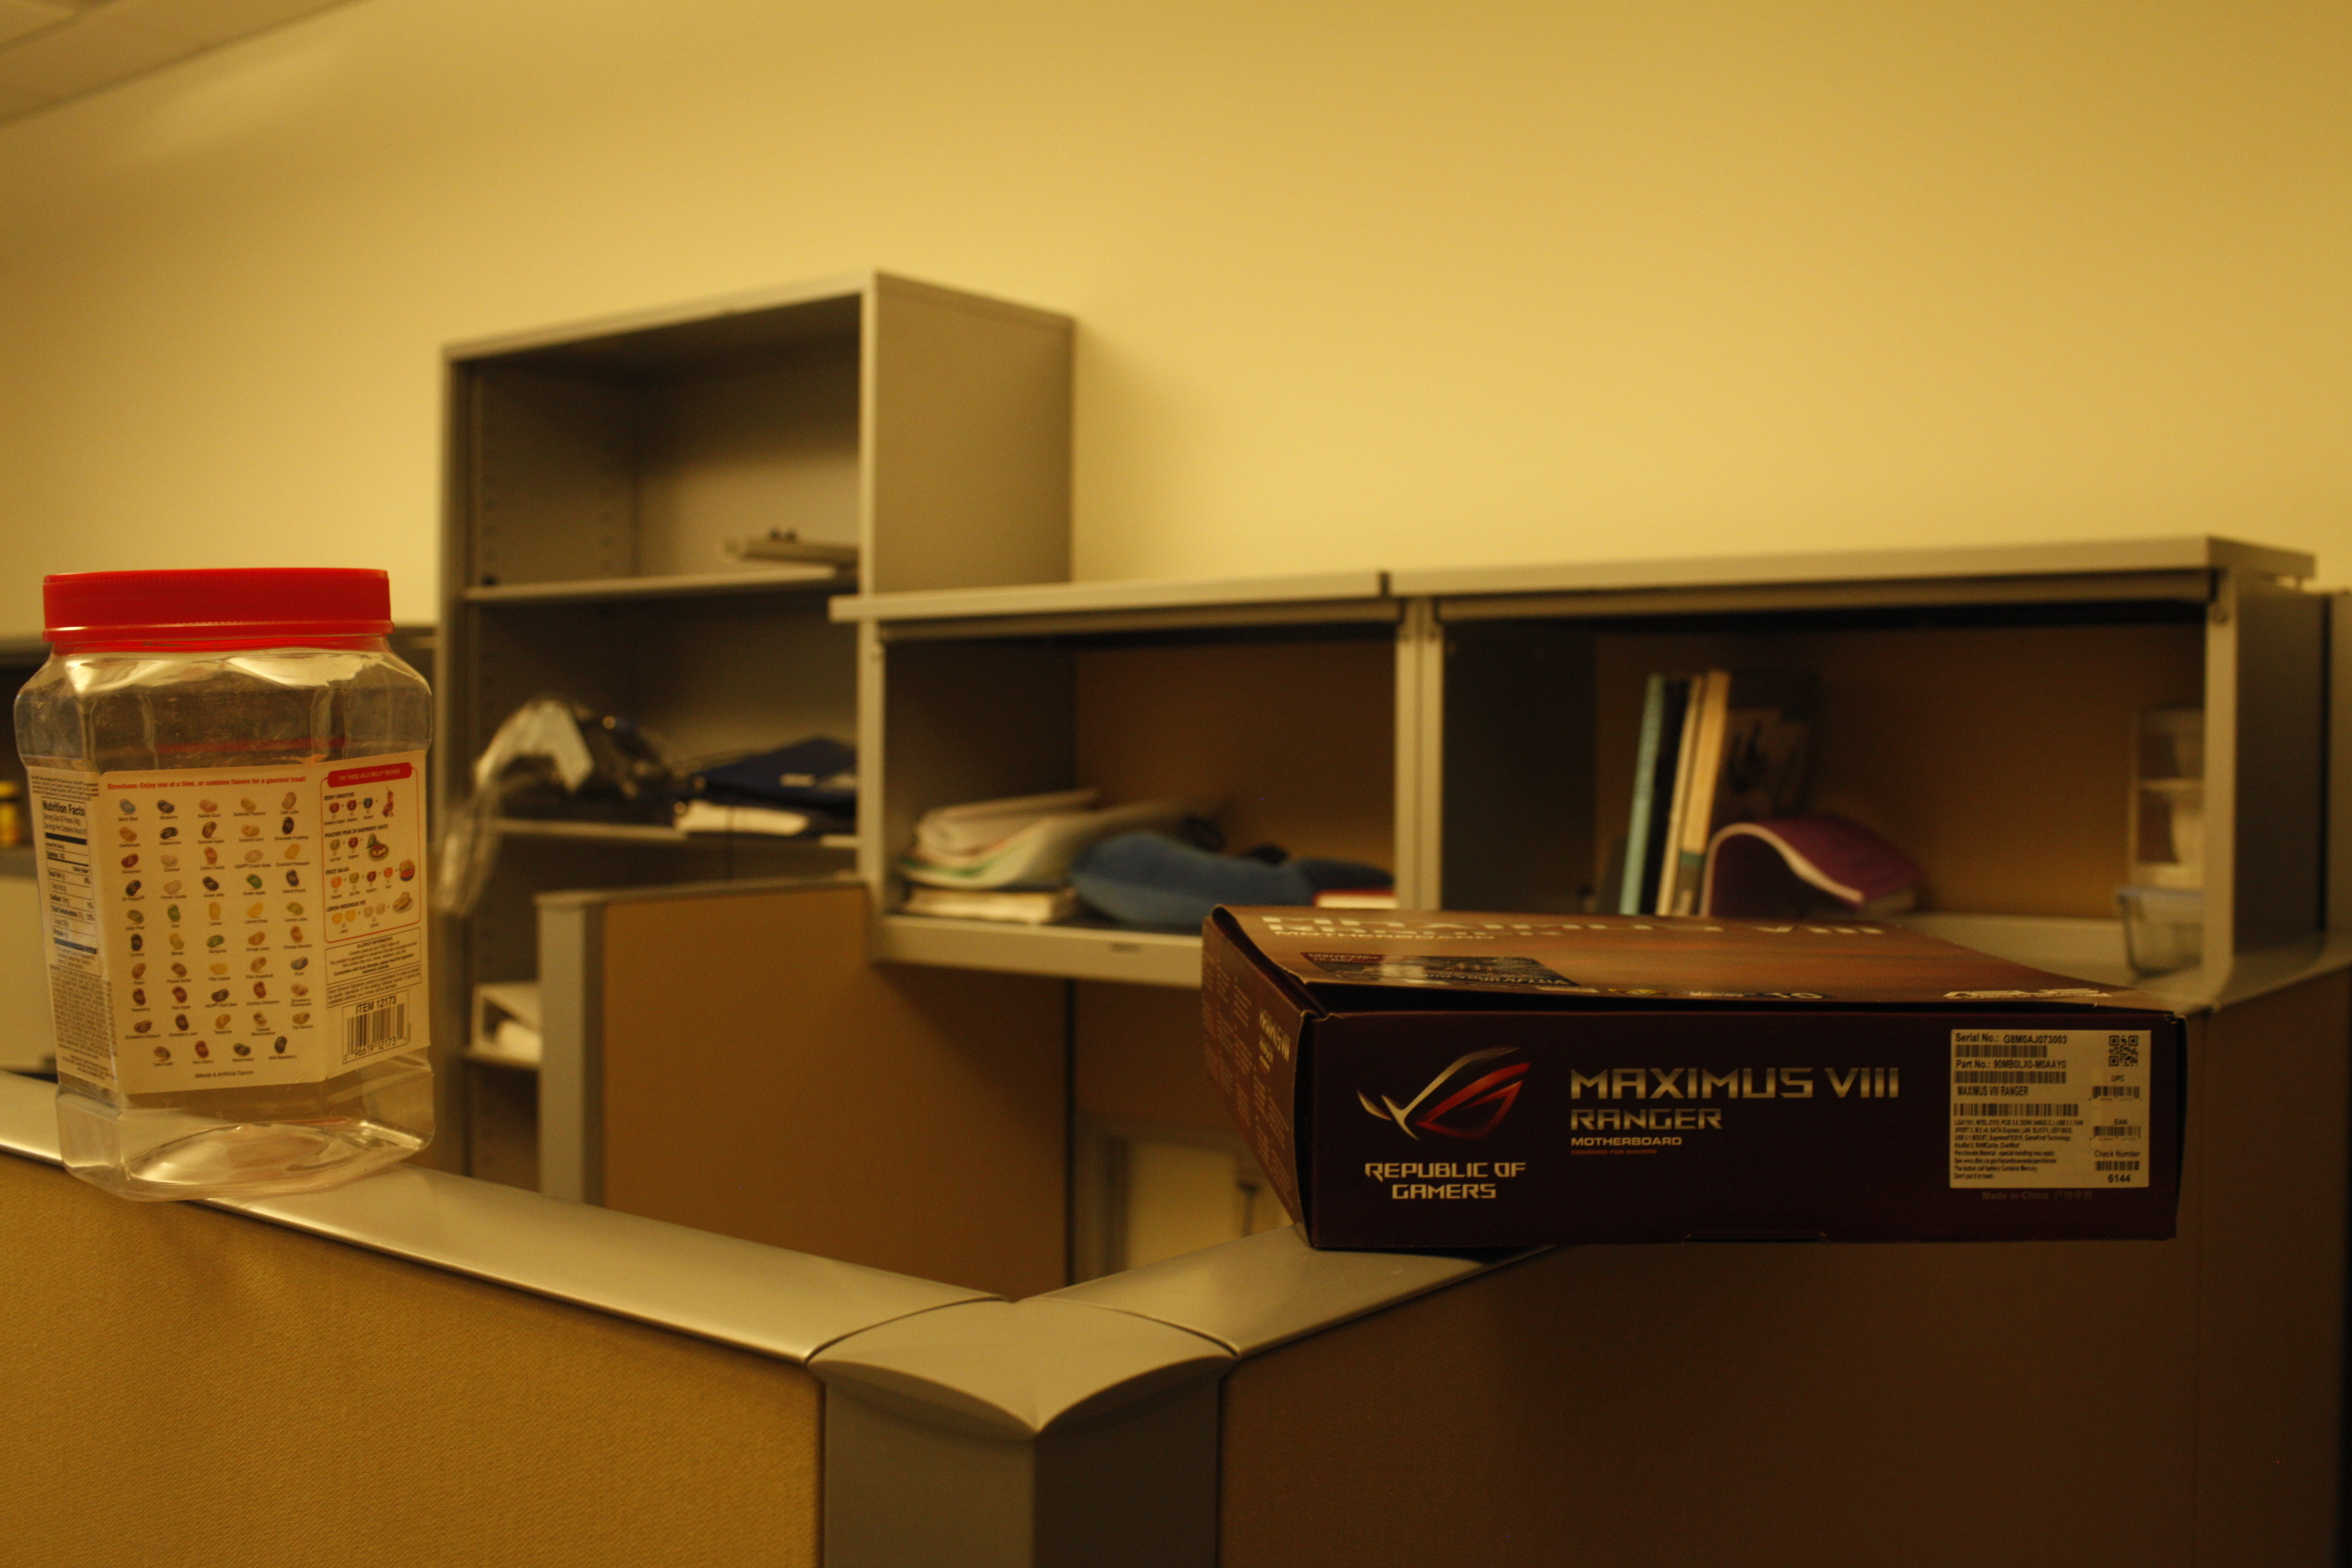
\includegraphics[width=.3\columnwidth]{images/multiview/p3}
}

\caption{Pictures taken from different distances and directions}
\label{fig:pictures}
\end{figure}

\section{Compute the essential matrix of all three camera pairs}

We first undistort pictures with calibration parameters as shown in Figure. There were 25 pixels loss in height and 12 pixels loss in width. Straight lines in those images confirms the calibration was done correctly.\\

In order to get pixel pairs over 3 camera pairs, we built a tool to allow us to pick those pixel pairs by hand. Figure \ref{fig:undistorted} shows the interface of our tool.\\

For each camera pair, we picked 17 to 18 pixel pairs to provide enough data calculating essential matrices and fundamental matrices. Figure \ref{fig:epipolar} shows the pixel pairs we picked over 3 camera pairs.\\

The essential matrices we calculated are

$$E_{12} =
\begin{bmatrix}
-2.944{\text e-}07&-1.993{\text e-}06&2.051{\text e-}02\\
3.242{\text e-}06&-9.280{\text e-}07&-2.045{\text e-}02\\
-2.030{\text e-}02&1.995{\text e-}02&1.000{\text e+}00 
\end{bmatrix}
$$

$$E_{13} =
\begin{bmatrix}
4.323{\text e-}08&1.144{\text e-}06&-1.610{\text e-}03\\
-2.850{\text e-}07&2.763{\text e-}07&-7.243{\text e-}03\\
5.939{\text e-}04&5.592{\text e-}03&1.000{\text e+}00
\end{bmatrix}
$$

$$E_{23} =
\begin{bmatrix}
1.608{\text e-}07&2.496{\text e-}07&-2.468{\text e-}03\\
-1.274{\text e-}07&1.268{\text e-}08&-1.230{\text e-}03\\
1.877{\text e-}03&9.439{\text e-}04&1.000{\text e+}00
\end{bmatrix}
$$


\begin{figure}[t]
\centering
\subfigure[Image 1]{
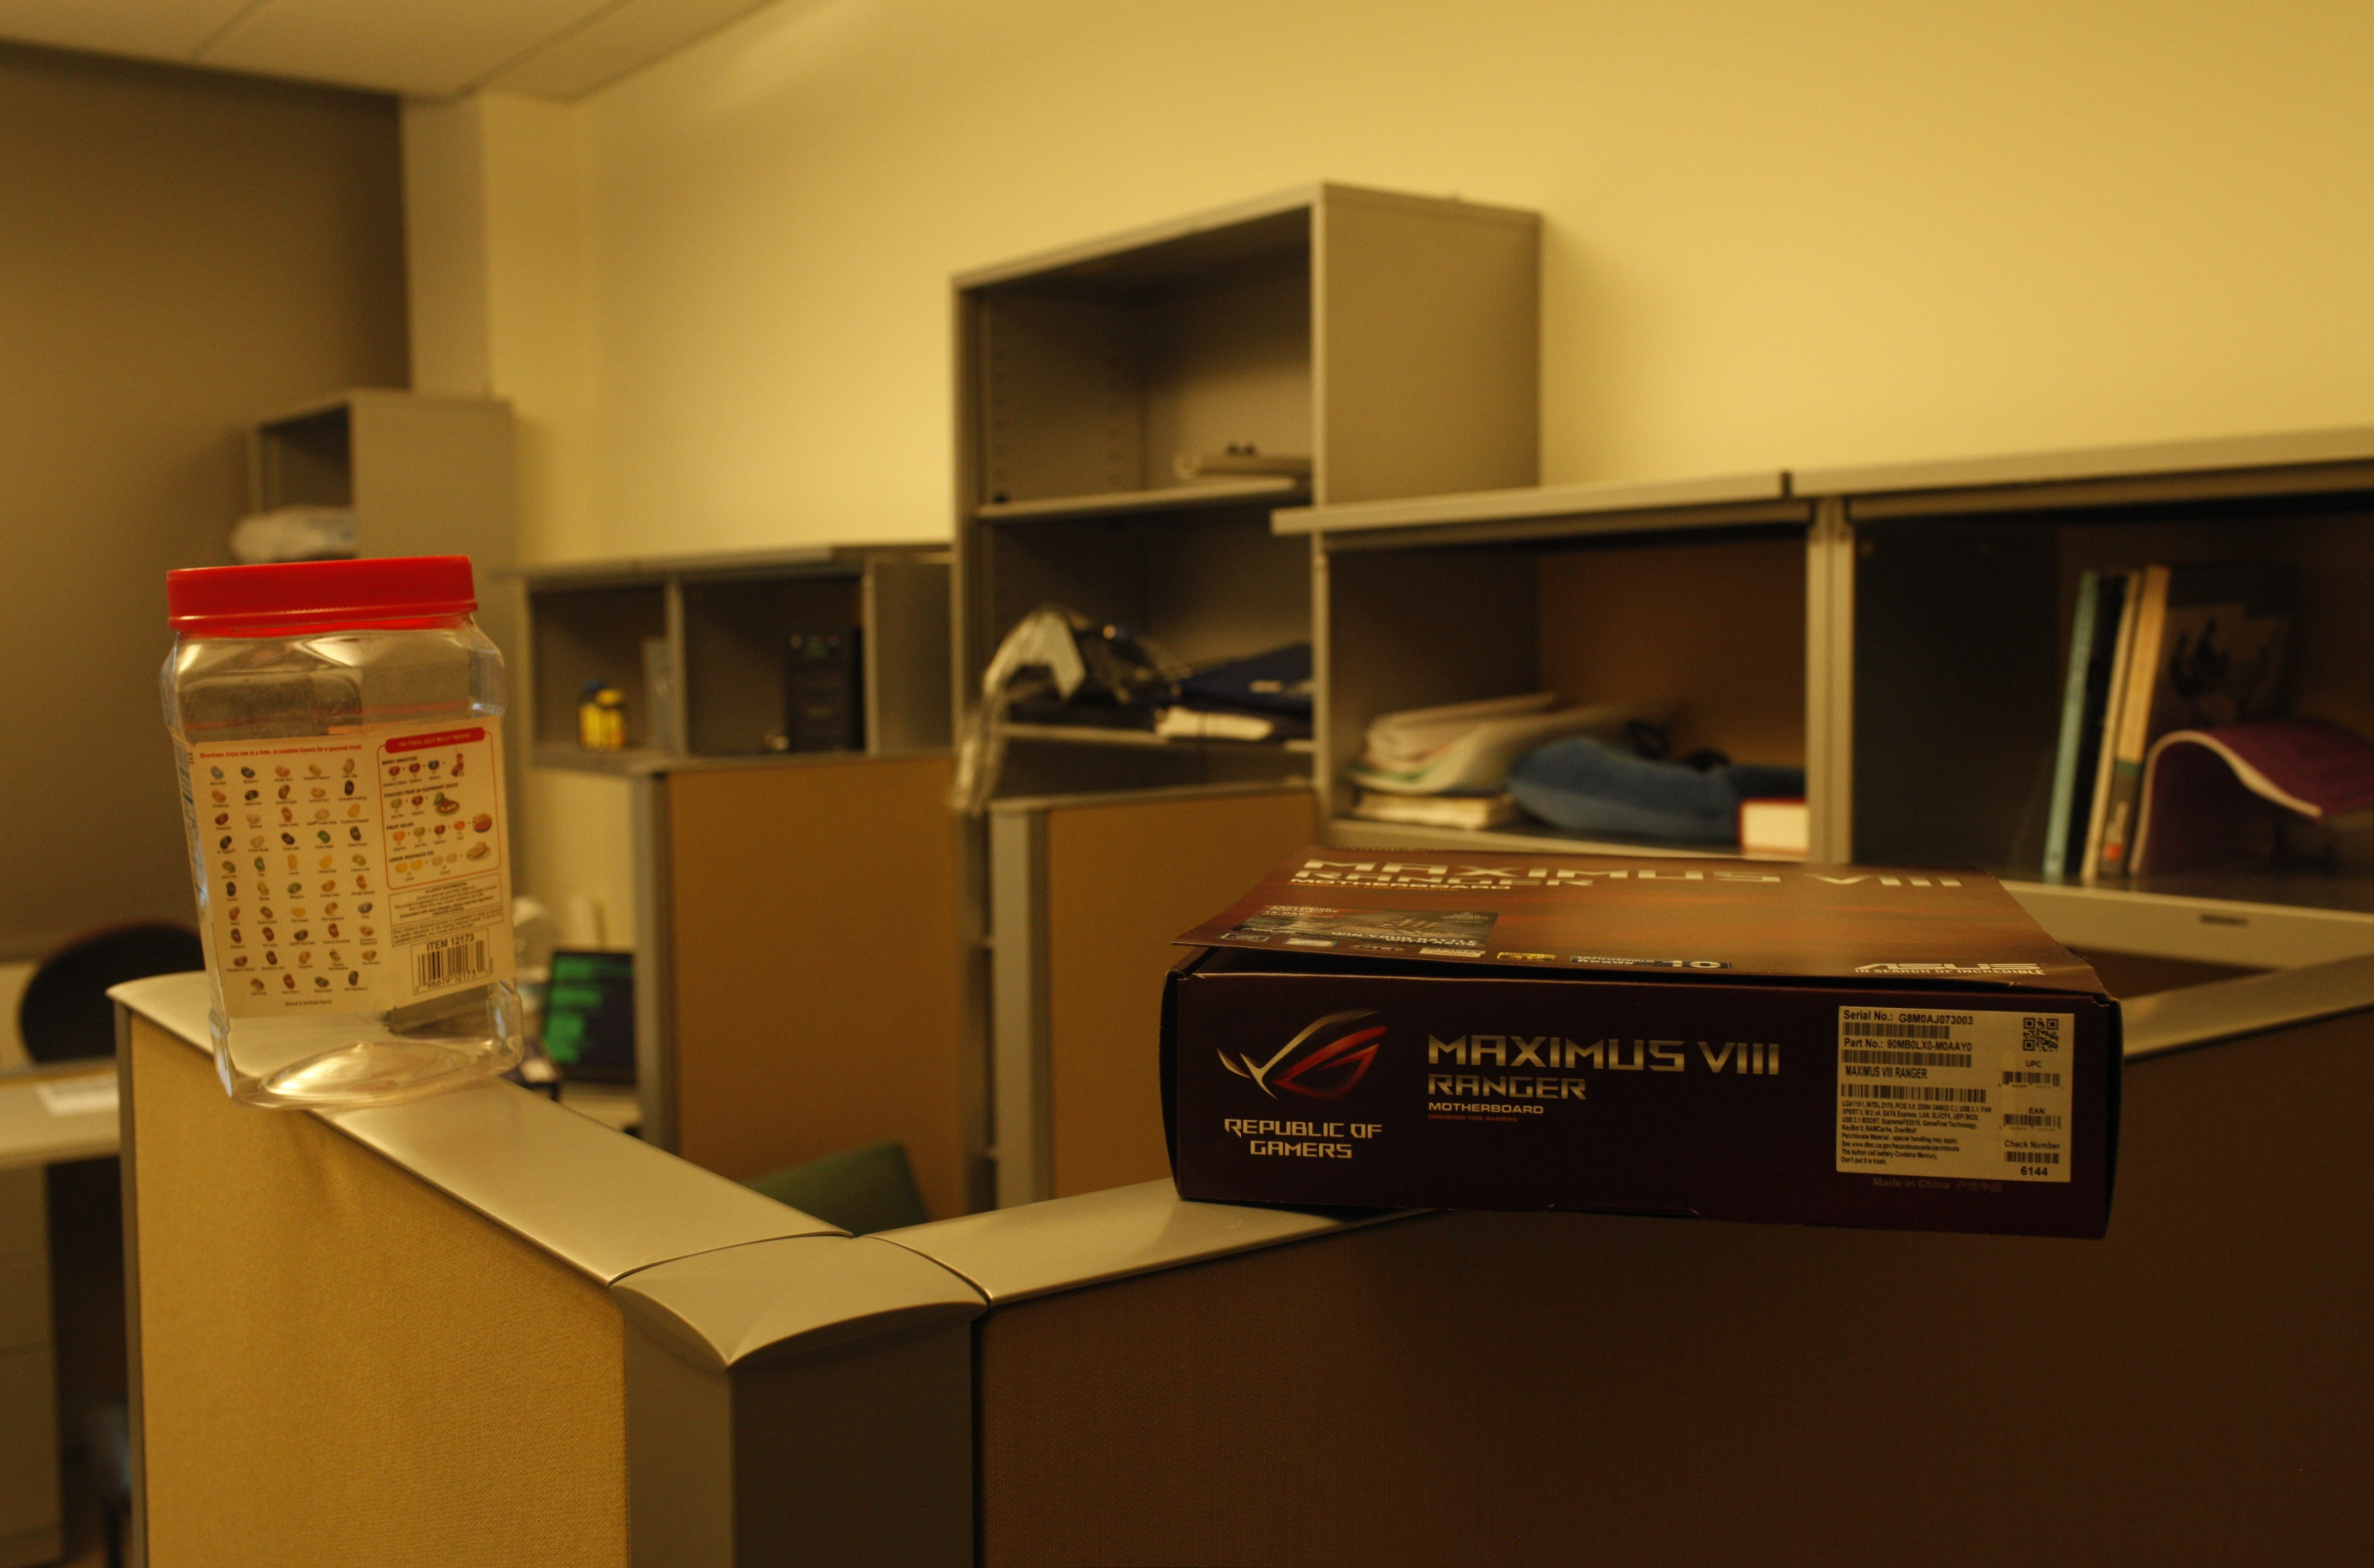
\includegraphics[width=.3\columnwidth]{images/undistorted/p1}
}
\subfigure[Image 2]{
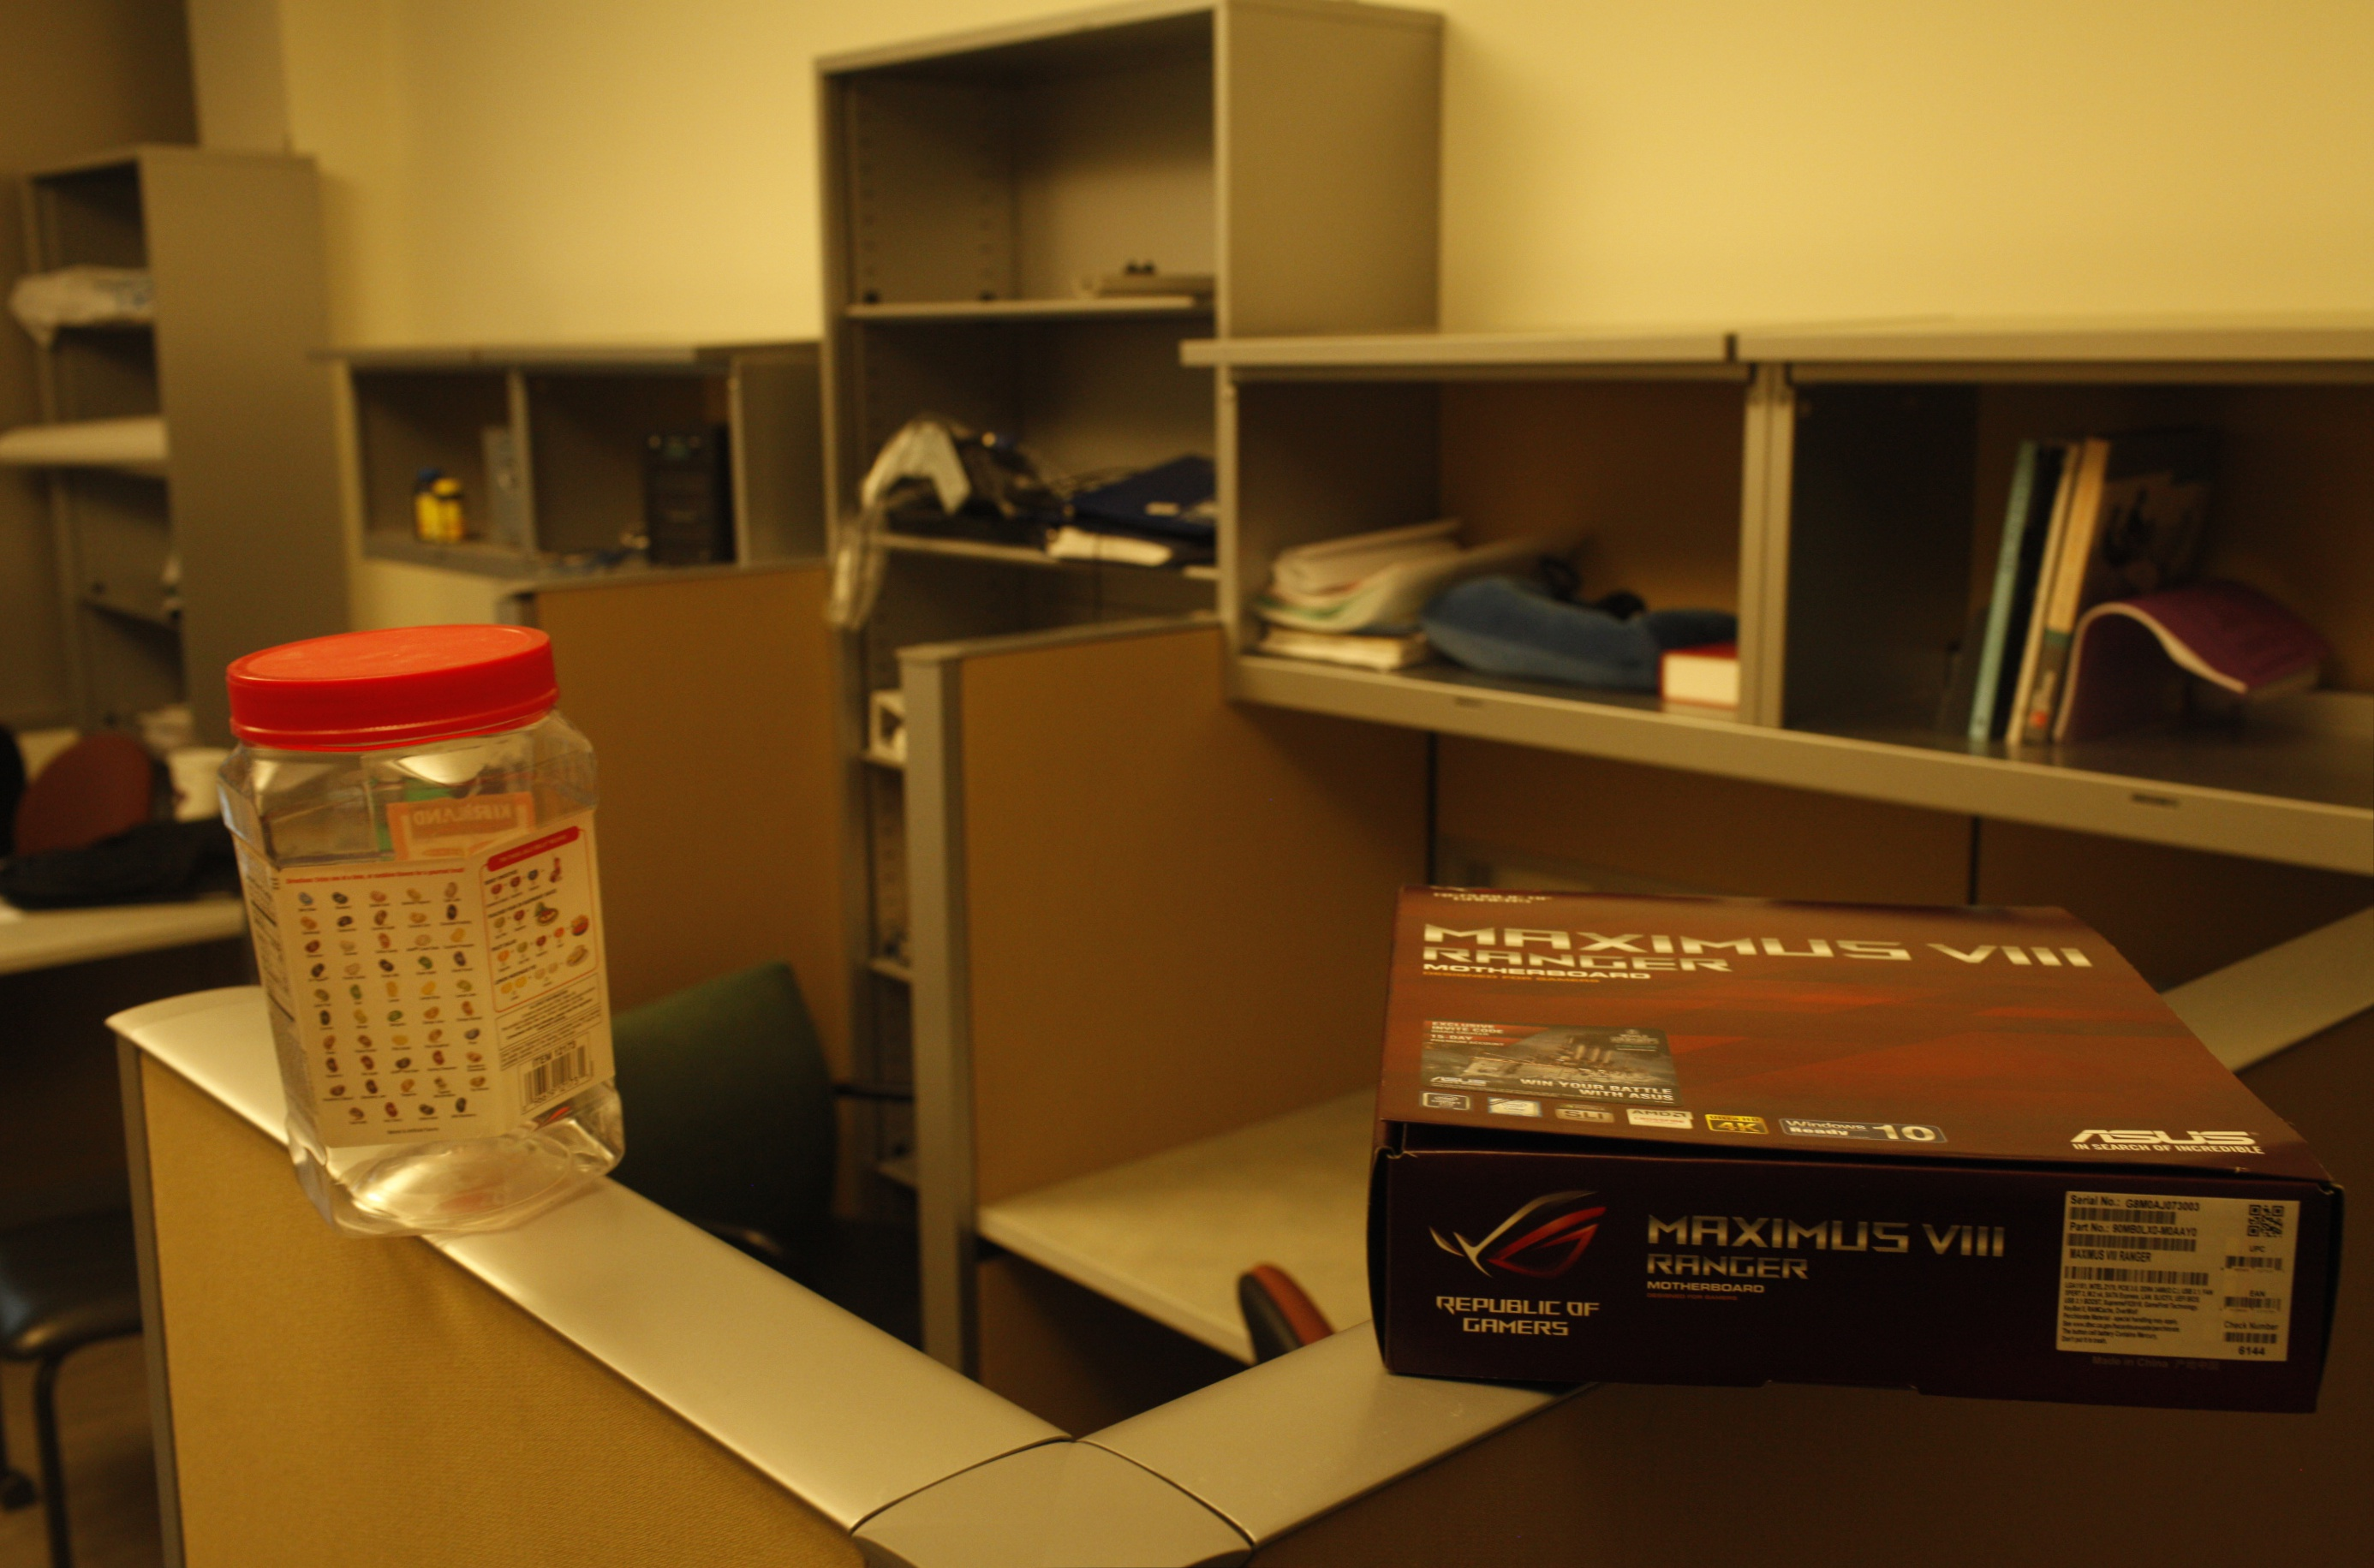
\includegraphics[width=.3\columnwidth]{images/undistorted/p2}
}
\subfigure[Image 3]{
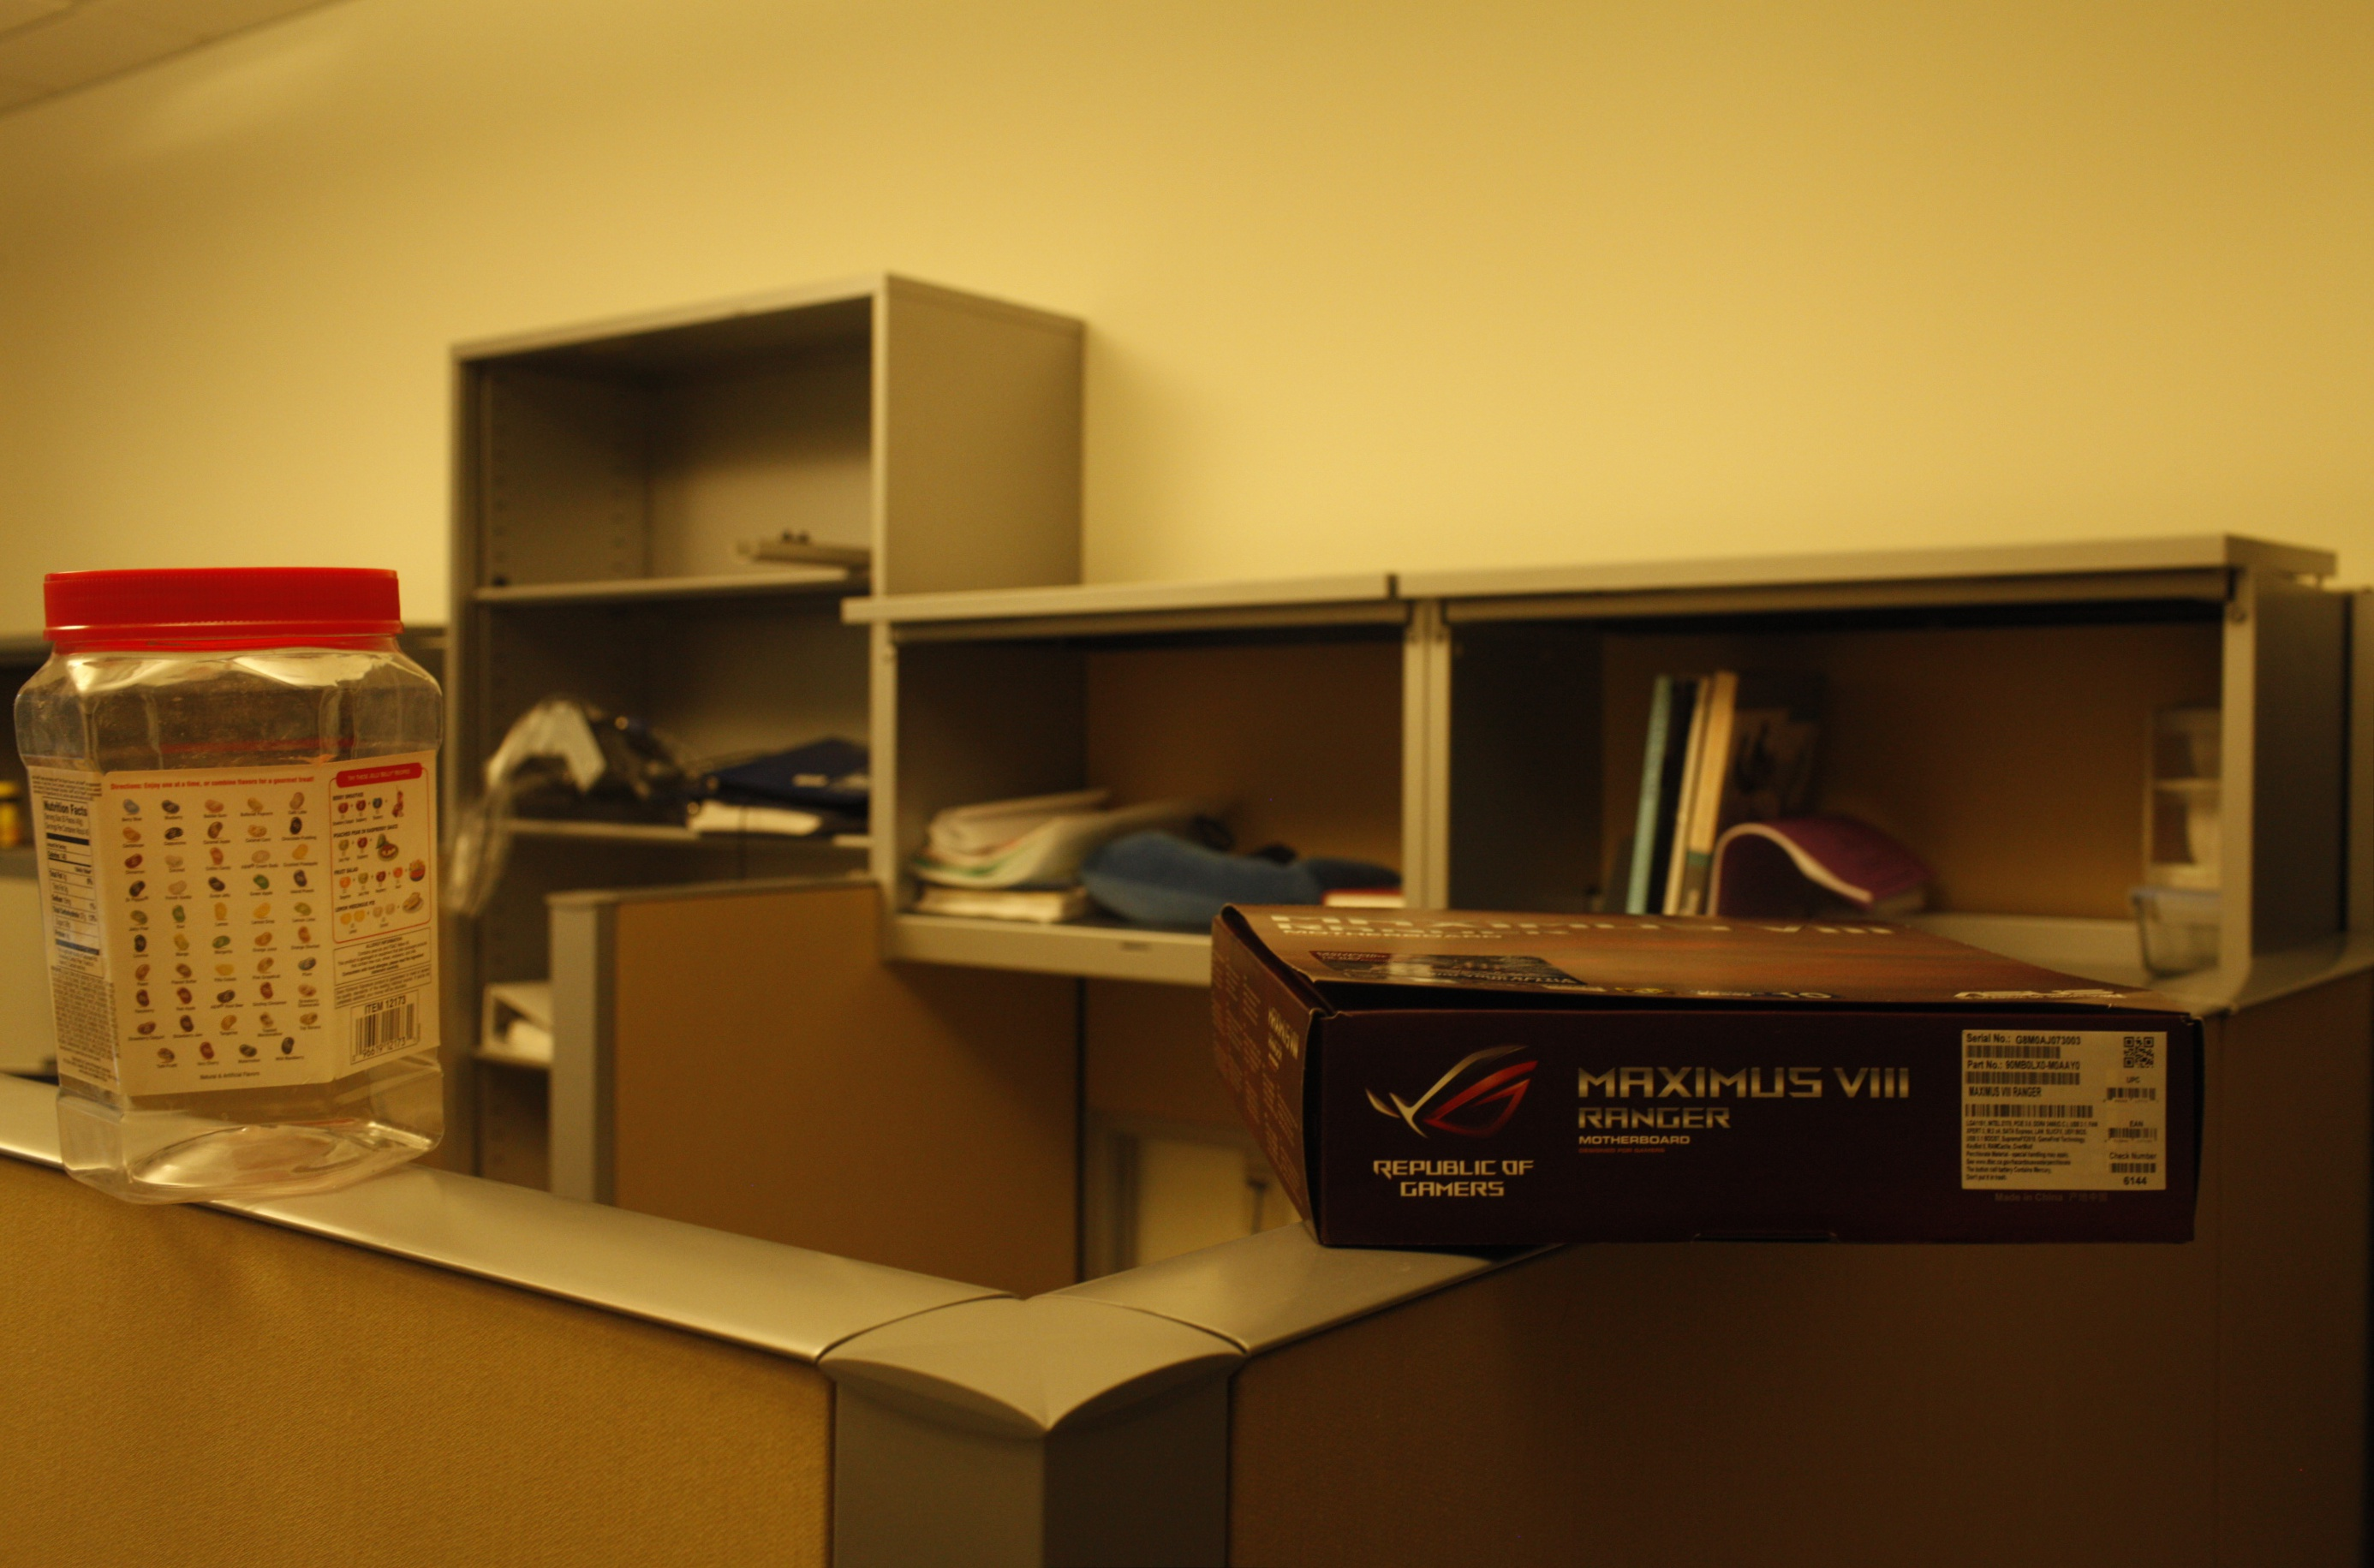
\includegraphics[width=.3\columnwidth]{images/undistorted/p3}
}

\caption{Undistorted pictures.}
\label{fig:undistorted}
\end{figure}


\begin{figure}[t]
\centering
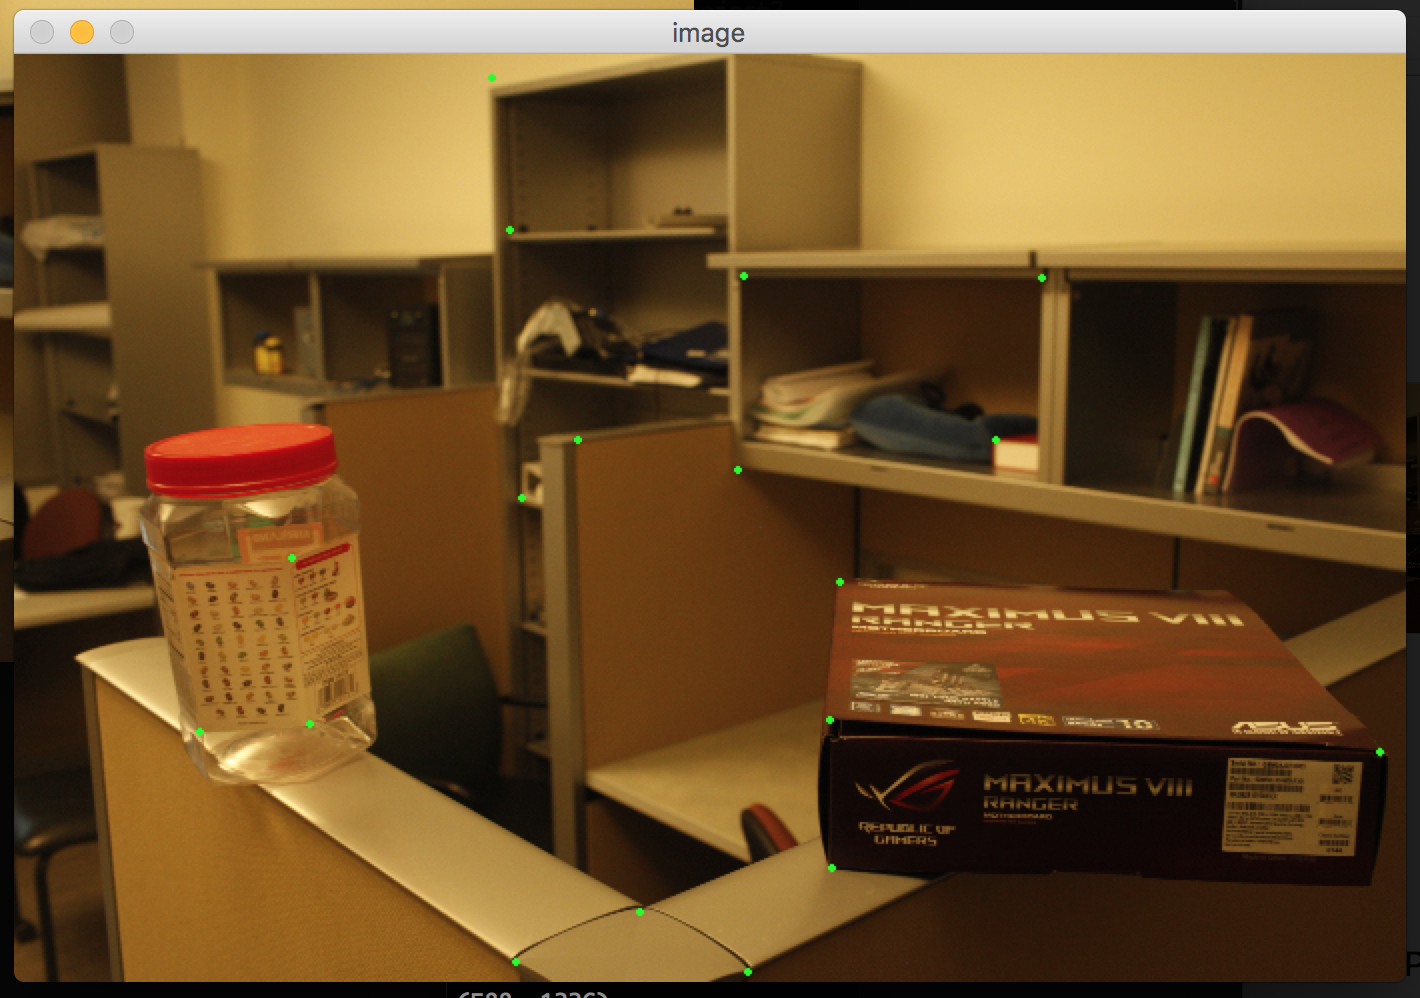
\includegraphics[width=\columnwidth]{images/pick}

\caption{Pictures taken from different distances and directions}
\label{fig:pick}
\end{figure}

\begin{figure}[t]
\centering
\subfigure[Image 1 - Image 2]{
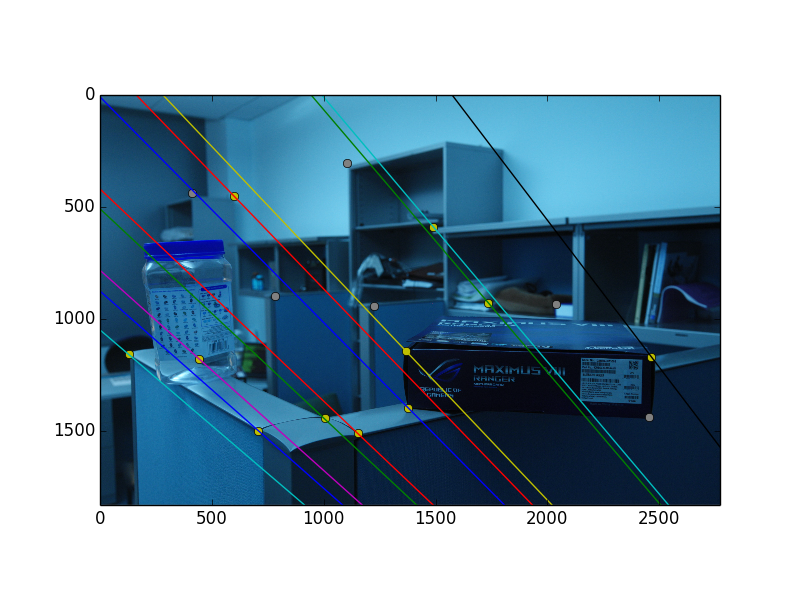
\includegraphics[width=.45\columnwidth]{images/epipolar/1-2-1}
}
\subfigure[Image 2 - Image 1]{
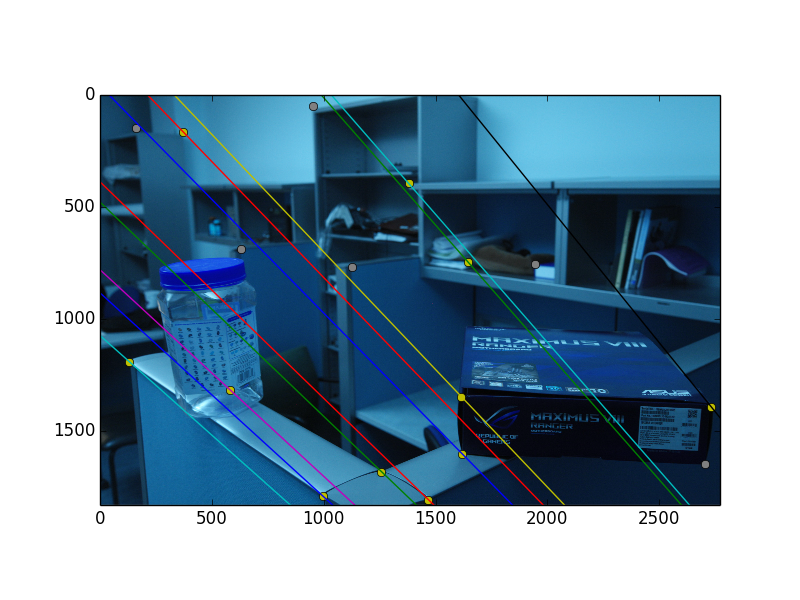
\includegraphics[width=.45\columnwidth]{images/epipolar/1-2-2}
}
\subfigure[Image 1 - Image 3]{
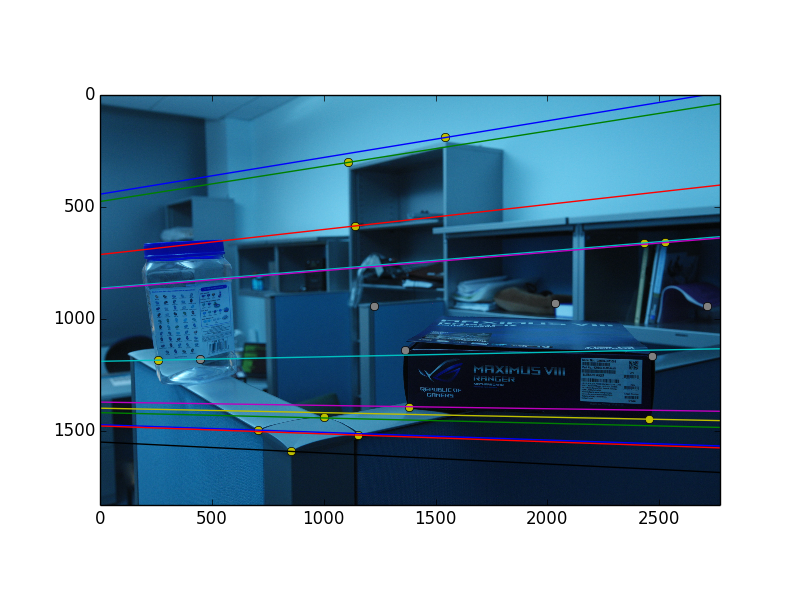
\includegraphics[width=.45\columnwidth]{images/epipolar/1-3-1}
}
\subfigure[Image 3 - Image 1]{
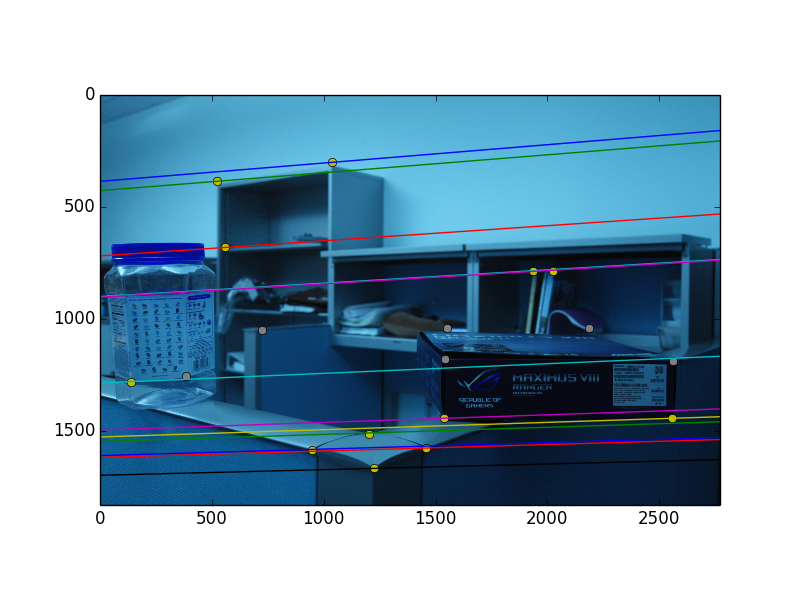
\includegraphics[width=.45\columnwidth]{images/epipolar/1-3-3}
}
\subfigure[Image 2 - Image 3]{
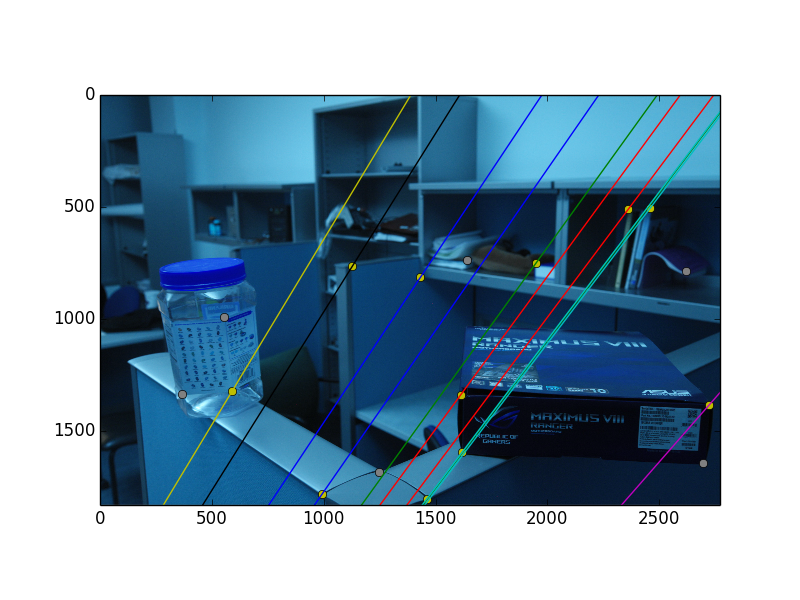
\includegraphics[width=.45\columnwidth]{images/epipolar/2-3-2}
}
\subfigure[Image 3 - Image 2]{
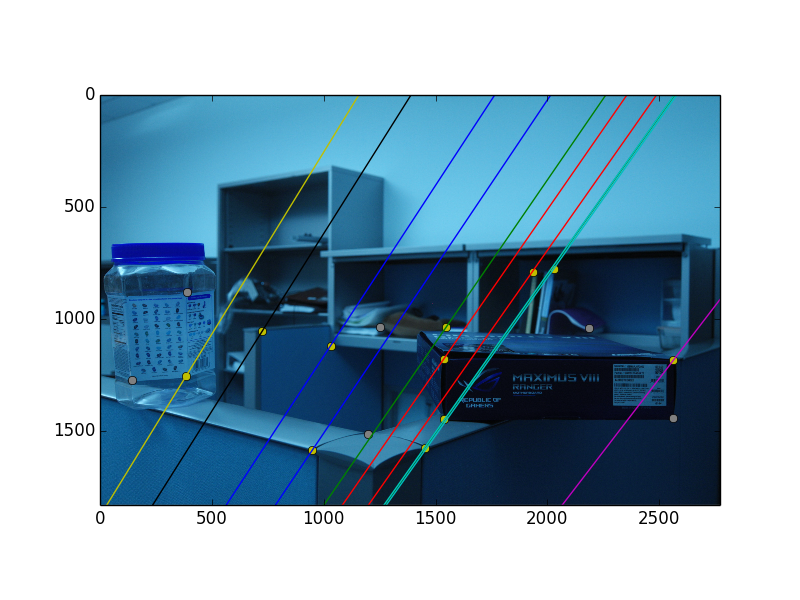
\includegraphics[width=.45\columnwidth]{images/epipolar/2-3-3}
}

\caption{Hand-pick pixel pairs (Inliers are yellow while outliers are gray) and corresponding epipolar lines.}
\label{fig:epipolar}
\end{figure}

\section{Acknowledgment}
We did all the project together. However, Ziqiang Wang is mainly responsible for
Section \ref{sec:create} and Section \ref{sec:reproduce} while Yanan Xie is responsible for the rest parts of this project including providing his professional photography devices.\\

Thanks to \LaTeX\ for providing such a great document preparation system. And many appreciates to the authors of Python, numpy, sklearn, OpenCV and matplotlib.\\



\end{document}
